Postępy w cyfryzacji ludzkich twarzy stały się podstawą nowoczesnych narzędzi do edycji obrazów twarzy. Narzędzia edycji można podzielić na dwie główne kategorie: modyfikację tożsamości i modyfikację wyrazu twarzy. Oprócz ręcznej edycji twarzy przy użyciu narzędzi takich jak Photoshop, w ostatnich latach zaproponowano wiele automatycznych podejść. Najbardziej znaczącą i powszechnie stosowaną techniką modyfikacji tożsamości jest zamiana twarzy, która zyskała znaczną popularność, ponieważ lekkie systemy są teraz zdolne do działania na telefonach komórkowych. Dodatkowo, dostępne są teraz techniki rekonstrukcji twarzy, które zmieniają wyraz twarzy osoby poprzez przeniesienie wyrazu źródłowej osoby na cel. Ninejsza praca przedswai dwa zautomatyzowane podjeścia deeepFake i Face2Face.

\subsection{DeepFake}
DeepFake to technologia, która wykorzystuje sztuczną inteligencję do tworzenia manipulacji wideo, w których twarze i głosy ludzi są zamieniane lub manipulowane w sposób realistyczny~\cite{DeepFakegithub}.
Przykad takiej podmiany pokazano na rysunku~\ref{img:deepfake-example}.
Termin `DeepFake' jest połączeniem słów `deep learning' (głębokie uczenie maszynowe) i `fake' (fałszywy), co odzwierciedla zastosowanie zaawansowanych algorytmów uczenia maszynowego w celu tworzenia realistycznych fałszerstw.

\begin{wrapfigure}{r}{0.5\textwidth}
    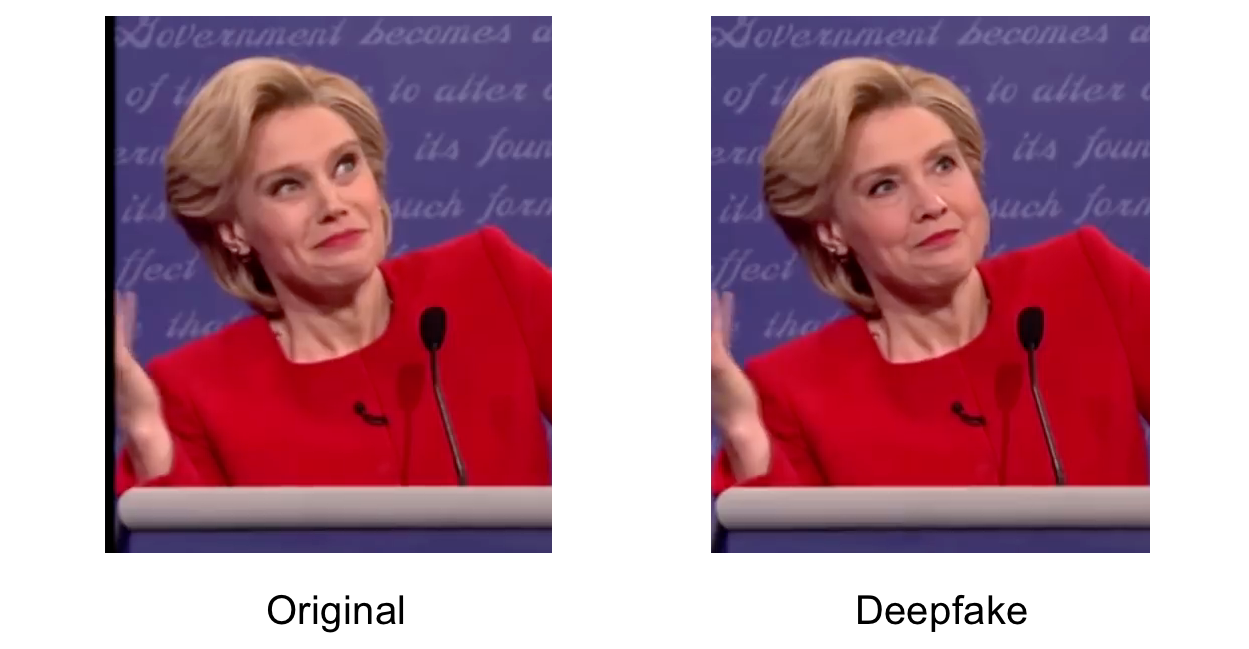
\includegraphics[width=\linewidth]{img/deepfake_example}
    \centering
    \caption{ Przykład zamiany twarzy za pomocą Deepfake. Zauważalny jest znaczny spadek ekspresyjności twarzy. Źródło:~\cite{mesoNet} }
    \label{img:deepfake-example}
\end{wrapfigure}

Głównym elementem technologii DeepFake jest sieć neuronowa, znana jako generatywna sieć przeciwnika (GAN)\cite{tolosana2020deepfakes}.
Proces tworzenia DeepFake zazwyczaj obejmuje dwa kluczowe etapy: trening i generację. W etapie treningowym sieć neuronowa jest uczona na dużej ilości danych, które zawierają pary obrazów i/lub nagrań dźwiękowych, reprezentujących oryginalne twarze i głosy osób, które mają zostać podmienione.
Na podstawie tych danych sieć neuronowa uczy się modelować charakterystyki twarzy i głosów.

Po etapie treningu następuje etap generacji, w którym sieć neuronowa jest używana do stworzenia nowego wideo, w którym twarze lub głosy są manipulowane.
Na podstawie podanych danych wejściowych (np. obrazów twarzy lub nagrania dźwiękowego), sieć generuje wideo, w którym twarze zostają podmienione na twarze osób z danych wejściowych lub głosy zostają podmienione na głosy innych osób. W rezultacie powstaje wideo, które wygląda i/lub słucha się tak, jakby osoba na wideo naprawdę mówiła lub miała określoną twarz.

DeepFake ma zarówno pozytywne, jak i negatywne aspekty. Z jednej strony może być wykorzystywany w dziedzinach takich jak przemysł filmowy, reklamowy czy rozrywkowy, aby tworzyć realistyczne efekty specjalne i efekty wizualne. Z drugiej strony, DeepFake może stanowić poważne zagrożenie, gdy jest wykorzystywany do oszustw, szantażu, fałszywych informacji, czy manipulacji politycznych.
Może wpływać na wiarygodność w mediach i stanowić wyzwanie dla autentyczności informacji.

Ze względu na swoje rosnące znaczenie i potencjalne zagrożenia, badania nad wykrywaniem DeepFake i opracowywanie metod rozpoznawania i ograniczania tego rodzaju manipulacji stają się coraz bardziej istotne dla bezpieczeństwa i zaufania wobec mediów i technologii cyfrowych.

\subsection{Face2Face}

Face2Face to system rekonstrukcji twarzy, który przenosi wyrażenia z wideo źródłowego na wideo docelowe, jednocześnie zachowując tożsamość osoby docelowej~\cite{thies2020face2face}.

\begin{figure}[h]
    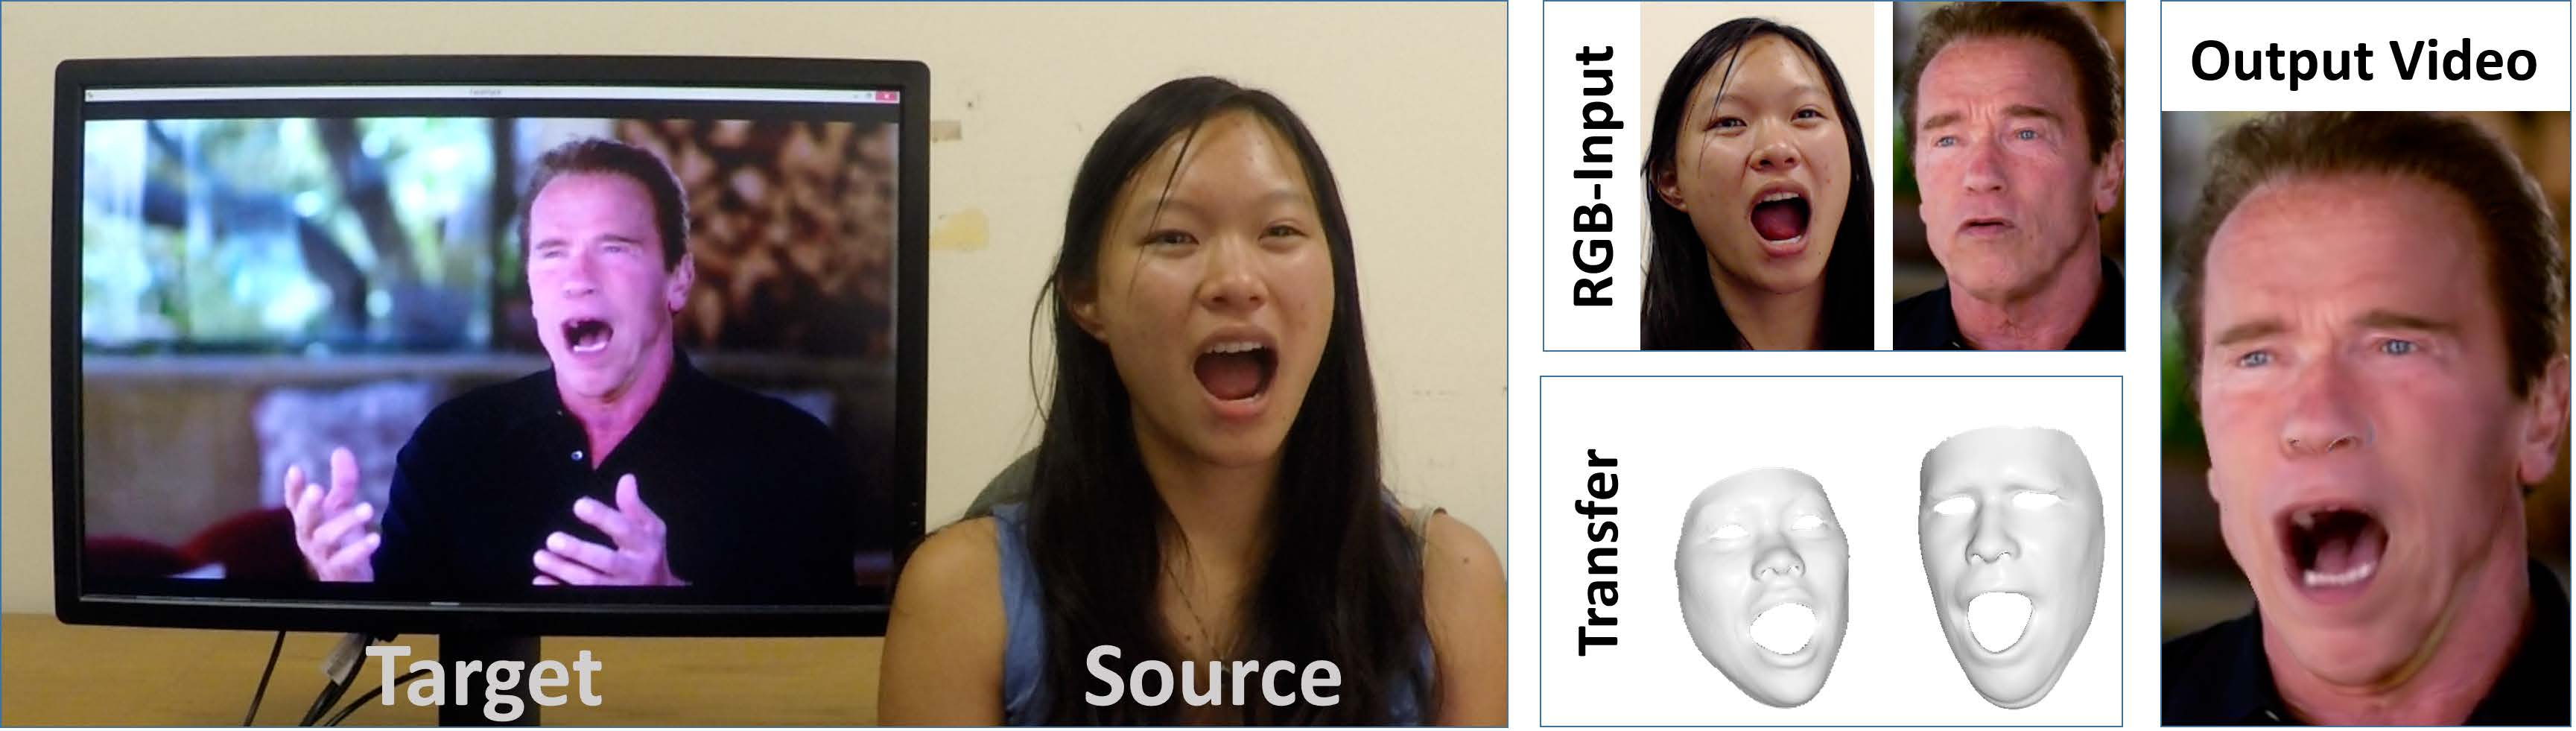
\includegraphics[width=0.9\linewidth]{img/Face2Face}
    \caption{ Działanie Face2Face Źródło:~\cite{thies2020face2face}}
    \label{img:face2face}
\end{figure}

Oryginalna implementacja Face2Face opiera się na dwóch strumieniach wideo, które są ręcznie wybierane jako kluczowe klatki.
Rysunek~\ref{img:face2face} pokazuje działanie omawianej technologi.
Twarz Arnolda Schwarzeneggera została zmieniona na bazie twarzy innej osoby.
Te klatki są wykorzystywane do generowania gęstej rekonstrukcji twarzy, która może być następnie użyta do odtworzenia twarzy przy różnym oświetleniu i wyrażeniach.
W pracy, dostosowujemy podejście Face2Face w celu automatycznego tworzenia manipulacji rekonstrukcyjnych.
Każde wideo jest przetwarzane w fazie wstępnej. Wykorzystujemy pierwsze klatki, aby uzyskać tymczasową tożsamość twarzy (czyli model 3D) i śledzimy wyrażenia na pozostałych klatkach. W celu wyboru kluczowych klatek wymaganych przez podejście, automatycznie wybieramy klatki z najbardziej skrajnym kątem twarzy. Na podstawie tej rekonstrukcji tożsamości śledzimy całe wideo, obliczając dla każdej klatki parametry wyrażenia, sztywnego położenia i oświetlenia, tak jak w oryginalnej implementacji Face2Face. Generujemy wynikowe wideo rekonstrukcji, przenosząc parametry wyrażeń źródłowych każdej klatki (czyli 76 współczynników Blendshape) na wideo docelowe. Szczegółowe informacje na temat procesu rekonstrukcji można znaleźć w oryginalnym artykule~\cite{thies2020face2face}.

Face2Face jest potężnym narzędziem, które umożliwia przenoszenie wyrażeń twarzy z jednego wideo na drugie, przy zachowaniu tożsamości osoby docelowej. Jego automatyczna wersja, zaimplementowana w ramach pracy, pozwala na masowe przetwarzanie wideo i tworzenie manipulacji rekonstrukcyjnych w sposób efektywny i skalowalny.

Badacze stosują nową, gęstą, bezmarkerową metodę przechwytywania wyrazu twarzy opartą na jednookularowych danych RGB, podobnie jak w najnowocześniejszych metodach. Jednak głównym wkładem jest odzwierciedlanie twarzy w czasie rzeczywistym, zamiast przekazywania wyrazu twarzy do wirtualnych postaci CG. W przeciwieństwie do poprzednich podejść do odzwierciedlania, które działają w trybie offline, celem jest przekazywanie wyrazu twarzy źródłowej osoby przechwyconej przez czujnik RGB do docelowej osoby w czasie rzeczywistym.
Docelowa sekwencja może być dowolnym wideo jednookularowym, na przykład wcześniejszym materiałem pobranym z serwisu YouTube z wyrazem twarzy. Celem jest modyfikacja docelowego wideo w fotorealistyczny sposób, tak aby manipulacje były praktycznie niemożliwe do zauważenia.
Wiernie fotorealistyczne odzwierciedlanie wyrazu twarzy stanowi podstawę wielu zastosowań, na przykład wideo-konferencji, gdzie strumień wideo może być dostosowany do ruchów twarzy tłumacza lub twarze mogą być przekonująco dubbingowane na język obcy.

W metodzie najpierw odtwarzana jest identyczność kształtu docelowej osoby za pomocą nowej globalnej, nieliniowej metody opartej na modelu, wykorzystując wcześniej nagrane sekwencje treningowe.
Ponieważ ten etap wstępny jest wykonywany globalnie na zestawie klatek treningowych, można rozwiązać niejednoznaczności geometryczne, które są typowe dla rekonstrukcji jednookularowej.
W czasie rzeczywistym śledzone są wyrazy twarzy zarówno osoby źródłowej, jak i docelowej przy użyciu metody analizy i syntezy opartej na statystycznym modelu wyrazu twarzy. Udowodniono, że dokładność śledzenia przy użyciu danych RGB jest porównywalna z najnowocześniejszymi metodami, nawet z metodami śledzenia online opartymi na danych głębi.
W celu przekazywania wyrazów twarzy od osoby źródłowej do docelowej w czasie rzeczywistym proponuje się nowe funkcje transferu, które skutecznie stosują transfer deformacji bezpośrednio w przestrzeni wyrazu twarzy o niskiej wymiarowości. Do ostatecznej syntezy obrazu odtwarzana jest twarz docelowej z przekazanymi współczynnikami wyrazu twarzy i komponowana jest z tłem wideo docelowej osoby z uwzględnieniem oszacowanego oświetlenia środowiska. Wprowadzana jest również nowa metoda syntezowania wnętrza ust oparta na obrazach, która generuje realistyczne wewnętrzne usta przez pobieranie i deformowanie najlepiej dopasowanych kształtów ust z wcześniej przygotowanej sekwencji próbkowania.
Ważne jest zauważenie, że zachowuje się wygląd kształtu ust docelowej osoby, podczas gdy istniejące metody albo kopiują obszar ust osoby źródłowej na docelową, albo renderują ogólny model zębów, co prowadzi do niejednoznacznych rezultatów.